\setAuthor{Jaan Kalda}
\setRound{lõppvoor}
\setYear{2012}
\setNumber{G 9}
\setDifficulty{8}
\setTopic{Elektrostaatika}

\prob{Laengud}
\begin{wrapfigure}{r}{0.33\textwidth}%
\vspace{-10pt}
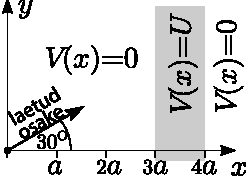
\includegraphics[width=\linewidth]{2012-v3g-09-laeng}%
\end{wrapfigure}
Positiivselt laetud osake kiirendatakse koordinaatide alguspunktis pinge $4U$ (kus $U>0$) abil teatud kiiruseni, mis
lebab $x-y$ tasandis $30$-kraadise nurga all $x$-telje suhtes, vt joonist. Elektriline potentsiaal $V(x,y)\equiv V(x)$
sõltub ainult $x$-koordinaadist: kui
$3a<x<4a$, siis $V(x)=U$ ning vastasel korral $V(x)=0$; peale elektrostaatilise jõu osakesele mingeid muid jõude ei mõju ning $a>0$.

\osa Visandage laengu trajektoor $x-y$-tasandis (geomeetrilisi mõõtmeid ja nurki pole vaja märkida).

\osa Nüüd on laetud osakeste allikaks koordinaatide alguspunktis asuv koaksiaalne vaakumdiood, mistõttu pinge $4U$
abil kiirendatud osakesi liigub isotroopselt (võrdsel hulgal) kõigis $x-y$-tasandi suundades;
$z$-suunaline kiiruskomponent on kõigil osakestel 0. Milline osa kõigist kiiratud osakestes jõuab ruumipiirkonda $x>4a$?

\hint
Kuivõrd potentsiaal sõltub ainult $x$-koordinaadist, on elektriväli kõikjal $x$-telje sihiline ning
impulsi $y$-komponent säilib. Täielik \enquote{sisepeegeldus} toimub siis, kui positiivse $x-$suunaga 
seotud kineetiline energia on suurem kui $qU$.

\solu
\osa Kuivõrd potentsiaal sõltub ainult $x$-koordinaadist, siis on elektriväli kõikjal $x$-telje sihiline ning
impulsi $y$-komponent säilib. Seega, kui osake siseneb kõrgema potentsiaaliga piirkonda, siis 
väheneb vaid kiiruse $x$-komponent ning
trajektoor on selline, nagu oleks valguskiirel optiliselt hõredamat kihti läbides.\\
\osa Täielik \enquote{sisepeegeldus} toimub siis, kui positiivse $x$-suunaga 
seotud kineetiline energia on suurem kui $qU$, mis vastab kiirusvektori 
ja $x$-telje vahelisele nugale
\[
\arccos \sqrt{\frac {qU}{4qU}}=\frac \pi 3.
\]
Ainult sellest nurgast väiksemate nurkade puhul saab osake läbida kõrgema 
potentsiaaliga kihti ning selliset osakeste suhteline hulk on
\[
\xi = \frac \pi 3 \div \pi = \frac 13.
\]

\probeng{Charges}
\begin{wrapfigure}{r}{0.33\textwidth}%
\vspace{-10pt}
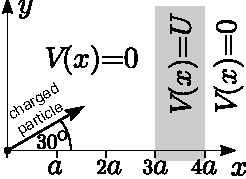
\includegraphics[width=\linewidth]{2012-v3g-09-laeng_ing}%
\end{wrapfigure}
A positively charged particle is accelerated from the origin with the help of a voltage $4U$ (where $U>0$) to a certain velocity which lies on the $x-y$ plane under the angle of $30$ degrees with respect to the $x$-axis (see figure). The electric potential $V(x,y)\equiv V(x)$ only depends on the $x$-coordinate: if $3a<x<4a$ then $V(x)=U$ and if not then $V(x)=0$; besides the electrostatic force no other forces are applied to the particle and $a>0$.\\
\osa Sketch the trajectory of the charge on the $x-y$ plane (you do not have to show the geometrical measurements or angles).\\
\osa The source of the charged particles is now a coaxial vacuum diode at the origin. Because of that the particles accelerated with the voltage $4U$ are moving isotropically (at equal quantities) to all directions of the $x-y$ plane; the $z$-directional component of the velocity for all particles is 0. What part of all the emitted particles reaches the region of space $x>4a$?

\hinteng
Since the potential only depends on the $x$-coordinate the electric field is $x$-directional everywhere and the $y$-component of the momentum remains. A total “internal reflection” occurs when the kinetic energy related to the positive $x-$-direction is bigger than $qU$.

\solueng
a) Since the potential only depends on the $x$-coordinate then the electric field is everywhere $x$-directional and the $y$-component of a momentum is preserved. Therefore if the particle enters a region with a higher potential then only the $x$-directional component of the velocity decreases and the trajectory is similar to the one a light ray would have when going through an optically less dense layer.\\
b) A complete internal reflection happens when the kinetic energy related to the positive $x$-direction is bigger than $qU$, which matches the angle between the velocity and the $x$-axis $\arccos \sqrt{\frac {qU}{4qU}}=\frac \pi 3$. Only for angles smaller than this angle can the particle go through a layer with a higher potential and the relative amount of such particles is $\xi = \frac \pi 3 \div \pi = \frac 13$.
\probend